\documentclass[12pt, titlepage]{article}

\usepackage{fullpage}
\usepackage[round]{natbib}
\usepackage{multirow}
\usepackage{booktabs}
\usepackage{tabularx}
\usepackage{graphicx}
\usepackage{float}
\usepackage{hyperref}
\hypersetup{
    colorlinks,
    citecolor=blue,
    filecolor=black,
    linkcolor=red,
    urlcolor=blue
}

\input{../../Comments.text}
\input{../../Common.text}

\newcounter{acnum}
\newcommand{\actheacnum}{AC\theacnum}
\newcommand{\acref}[1]{AC\ref{#1}}

\newcounter{ucnum}
\newcommand{\uctheucnum}{UC\theucnum}
\newcommand{\uref}[1]{UC\ref{#1}}

\newcounter{mnum}
\newcommand{\mthemnum}{M\themnum}
\newcommand{\mref}[1]{M\ref{#1}}

\begin{document}

\title{Interfaces Proposal for \progname{}} 
\author{\authname}
\date{\today}

\maketitle

\pagenumbering{roman}


\newpage

\tableofcontents


\listoffigures

\newpage

\pagenumbering{arabic}

\section{Introduction}
\section{Introduction}

This document presents the wireframes for \progname{}. Wireframes are low-fidelity visual layouts that show the structure, content, and functionality of each interface without the detail of a final design. They serve as a blueprint for the user interface and guide its implementation, ensuring that the team shares a clear understanding of how the system will look and behave.

The wireframes were created based on the project specification, so that each interface supports the functionality and requirements the system is expected to meet. Once the initial designs were complete, they were reviewed by our supervisors, who provided feedback on how the interfaces could be improved. The corresponding changes were then made, and the final versions are presented in this document.

This document covers the following interfaces:

\begin{itemize}
    \item Individual Assessment Interface
    \item Individual Question Interface
    \item Annotation Tool Interface
    \item Report Generation Interface
    \item Patient Summary Interface
\end{itemize}

\section{Introduction}

This document presents the wireframes for \progname{}. Wireframes are low-fidelity visual layouts that show the structure, content, and functionality of each interface without the detail of a final design. 
They serve as a blueprint for the user interface and guide its implementation, ensuring that the team shares a clear understanding of how the system will look and behave.

The wireframes were created based on the project specification, so that each interface supports the functionality and requirements the system is expected to meet \citep{SRS}. 
Once the initial designs were complete, they were reviewed by our supervisors, who provided feedback on how the interfaces could be improved. The corresponding changes were then made, and the final versions are presented in this document.

This document covers the following interfaces:

\begin{itemize}
    \item Individual Assessment Interface
    \item Individual Question Interface
    \item Annotation Tool Interface
    \item Report Generation Interface
    \item Patient Summary Interface
\end{itemize}

Each interface is shown in its own section, along with any changes made after the supervisor review and the reasoning behind them.



\section{Individual Assessment Page}
The individual assessment page gives clinicians an overview of a patient’s assessment, including its date and overall score. As shown in Figure~\ref{individual_assessment_view}, the left panel contains the assessment recording, transcript status, and space for assessment notes. The right panel summarizes verified, unverified, and flagged responses, followed by question rows showing answer outcomes, timestamps, verification statuses, and flag indicators. Clinicians can open questions for a detailed review, access the full assessment in SAFA, or generate a report.
\begin{figure}[H]
    \centering
    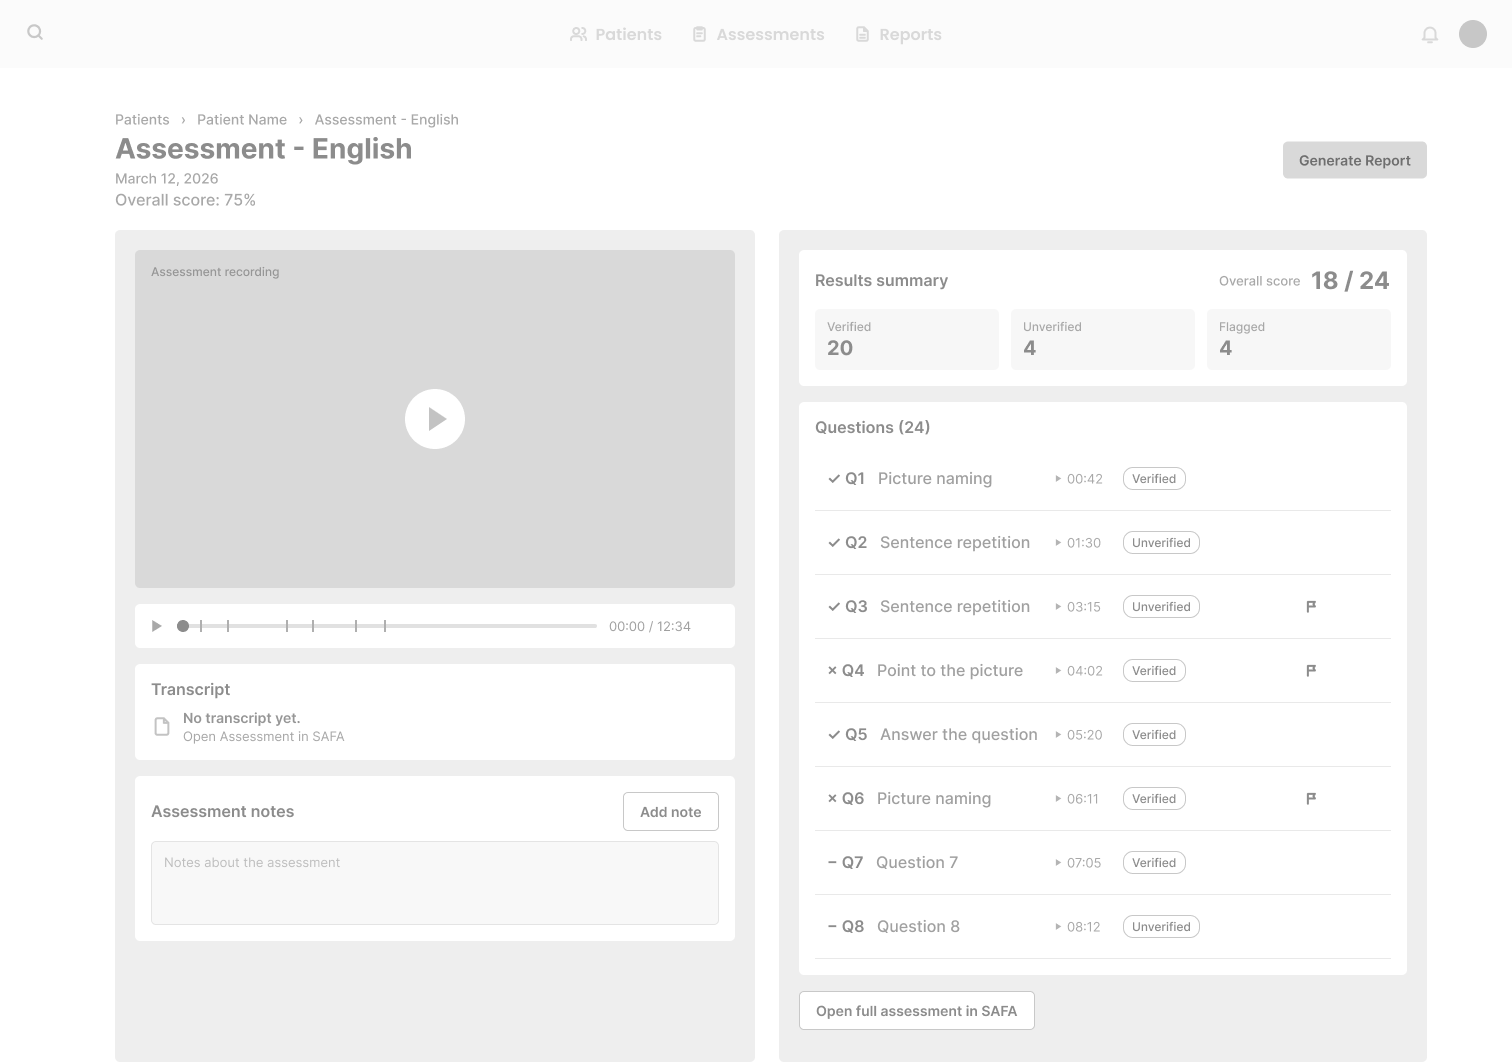
\includegraphics[width=\textwidth]{Images/individual_assessment_page_1.png}
    \caption{Individual Assessment View }
    \label{individual_assessment_view}
\end{figure}

\noindent After consulting with the supervisors, it was determined that the page contained all necessary functions and had a clear, easy-to-navigate UI. Hence, no changes were made to the design, and it will be used as is for implementation.


\section{Individual Question Page}
The individual question view was designed such that it supports detailed review of a single question. 
As shown in Figure~\ref{individual_question_view_alpha}, initially, the page’s content and clinician controls were tailored to the question type. In this case, clinicians can listen to the question and the patient’s recorded answer, then mark the response as correct, neutral, or incorrect. 
They can also review the relevant recording, update verification, flag interference, and add question-specific notes. Navigation allows them to move between questions or return to the assessment overview.

\begin{figure}[H]
    \centering
    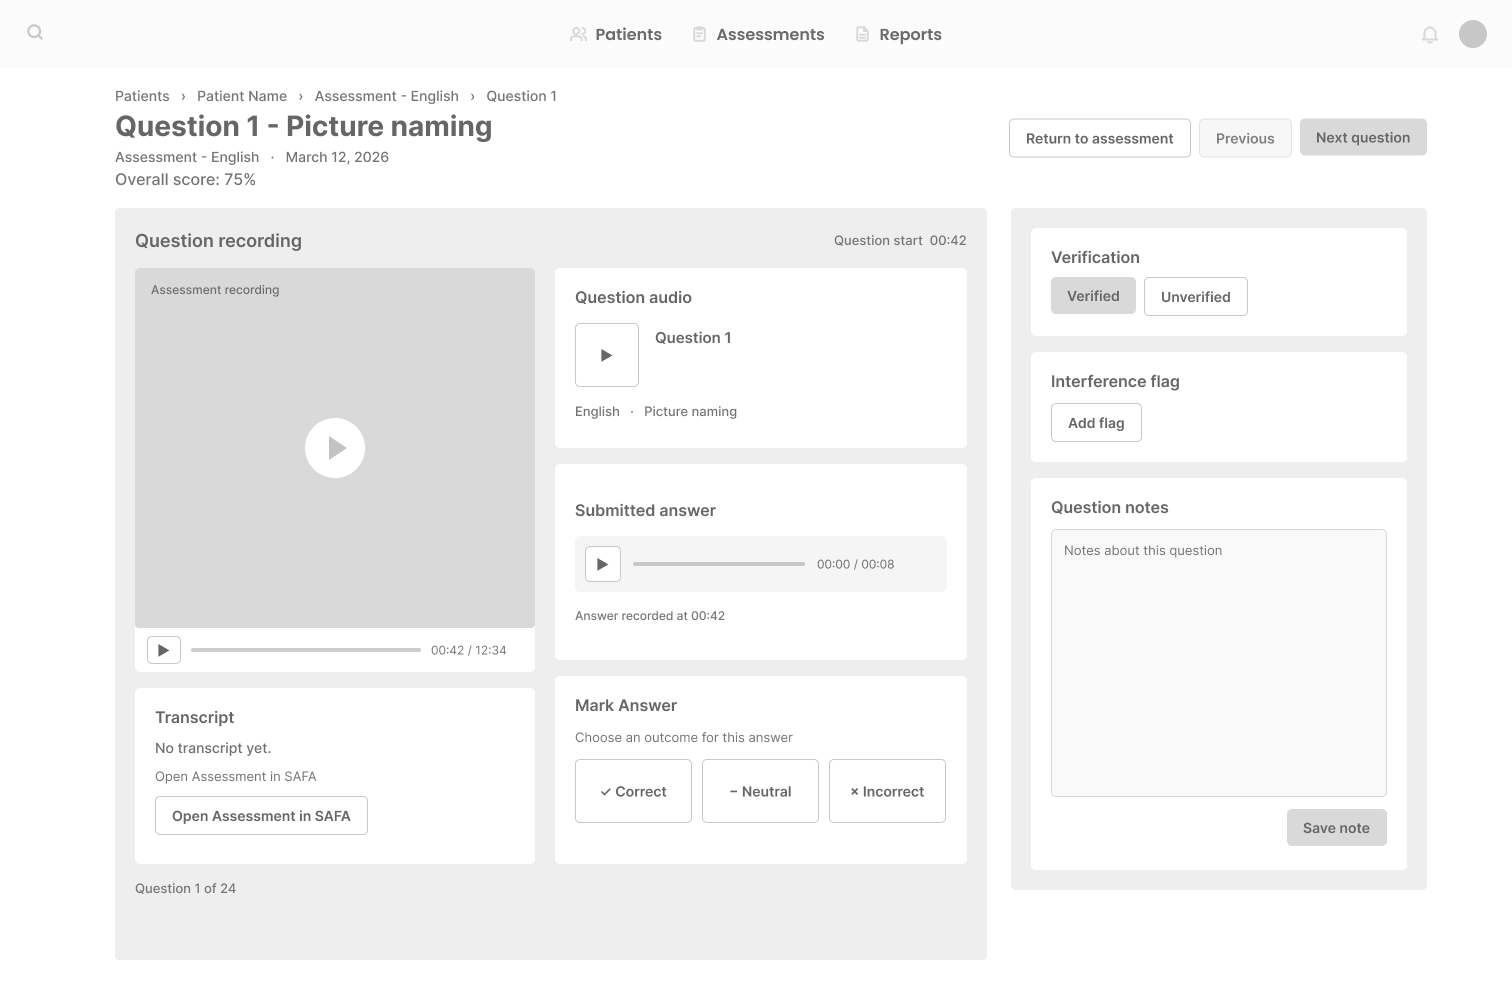
\includegraphics[width=\textwidth]{Images/individual_question_view_1-alpha.png}
    \caption{Initial Design of the Individual Question View }
    \label{individual_question_view_alpha}
\end{figure}

\noindent After consulting with the project supervisor, it was recommended that the interface be simplified to further streamline the clinician workflow. The following changes were made, along with the reasoning behind each.
\begin{enumerate}
    \item \textbf{Suggested Change:} Remove the video playback and the audio playback of both the question and the answer.

    \textbf{Reason and Result:} This streamlines the clinician's workflow, since they no longer need to listen to the question and can instead read the auto-generated transcript. As shown in Figure~\ref{individual_question_view}, the Question Audio and Submitted Answer views have been replaced by text-based Question and Answer views, which are now larger.

    \item \textbf{Suggested Change:} Remove the panel containing the Verification, Interference Flag, and Question Notes cards from the base UI, and instead let the clinician open it as a pop-up window.

    \textbf{Reason and Result:} This reduces on-screen clutter and keeps the clinician's most important functions easy to access and use. As shown in Figure~\ref{individual_question_view_with_interference}, a button on the right-hand side of the screen now opens the window. Figure~\ref{individual_question_view_with_flagged_interference} shows the UI after the Interference button is clicked and the window opens. 

\end{enumerate}


\begin{figure}[H]
    \centering
    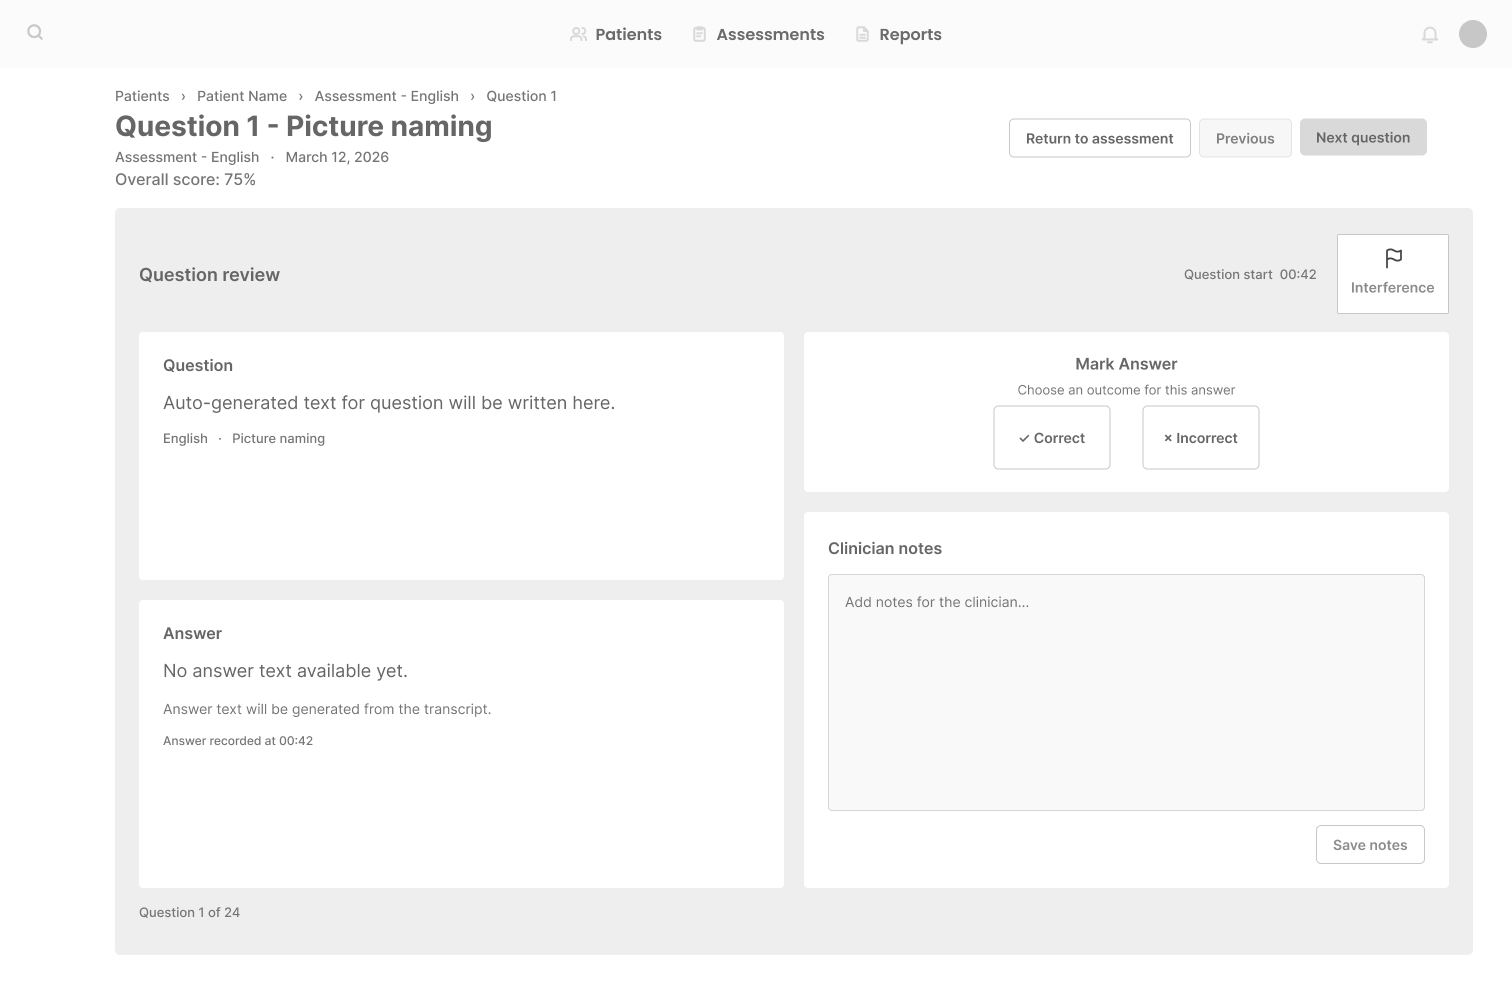
\includegraphics[width=\textwidth]{Images/individual_question_view_1}
    \caption{Individual Question View }
    \label{individual_question_view}
\end{figure}

\begin{figure}[H]
    \centering
    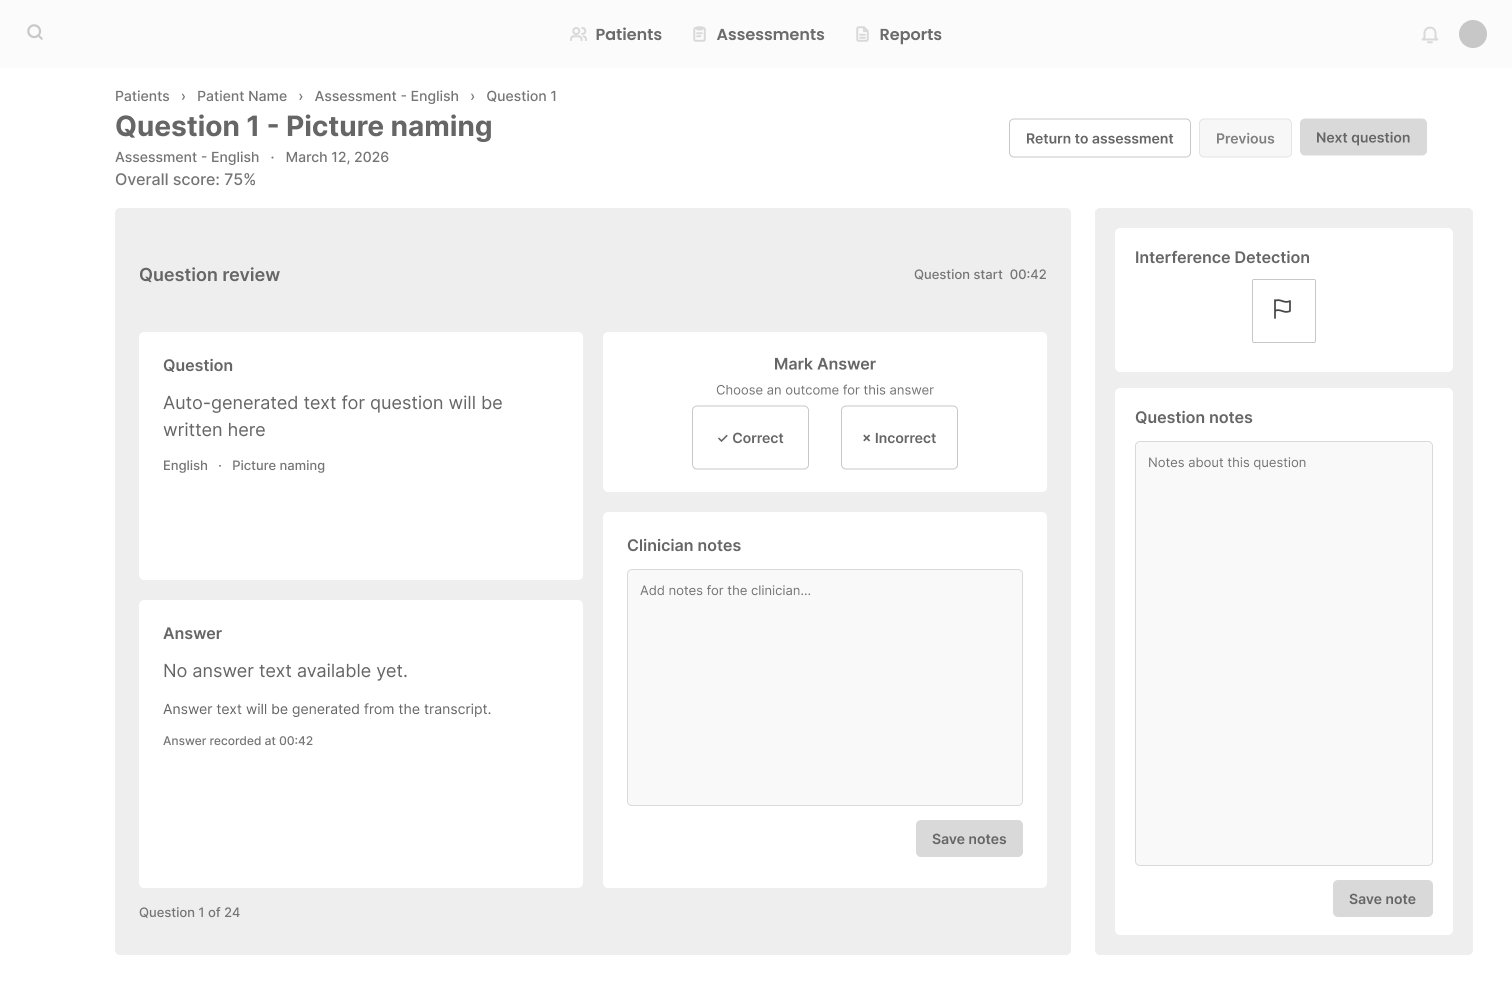
\includegraphics[width=\textwidth]{Images/individual_question_view_2}
    \caption{Individual Question View With Interference View Open and Unflagged}
    \label{individual_question_view_with_interference}
\end{figure}

\begin{figure}[H]
    \centering
    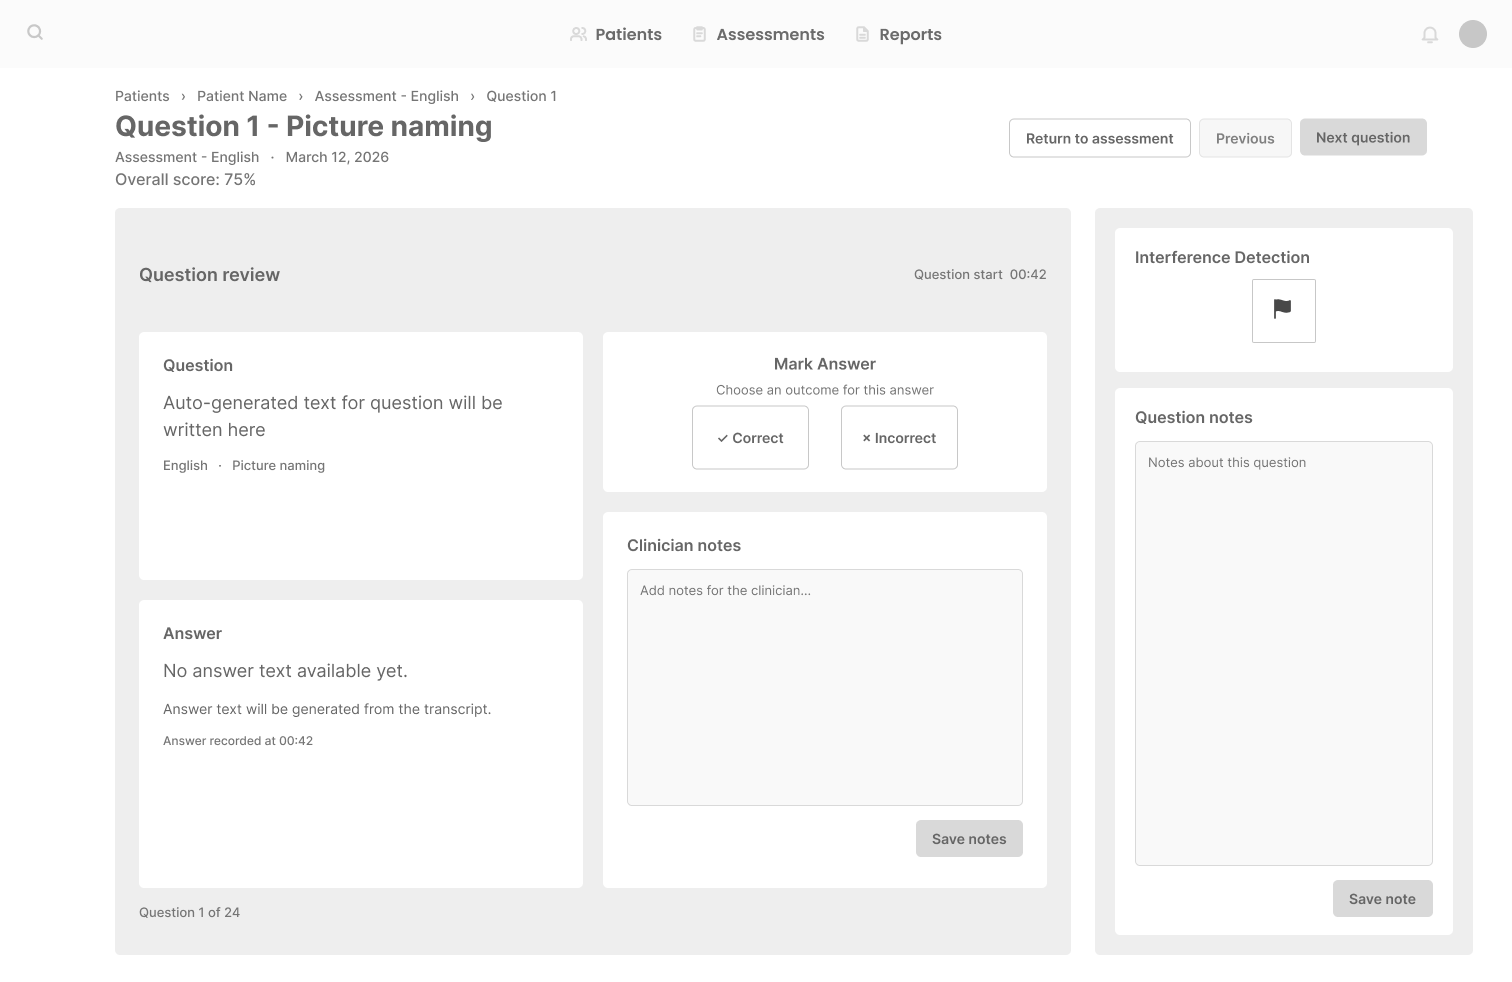
\includegraphics[width=\textwidth]{Images/individual_question_view_3-interference_flagged.png}
    \caption{Individual Question View With Interference View Open and Flagged}
    \label{individual_question_view_with_flagged_interference}
\end{figure}

\section{Annotation Tool Interface}

\section{Report Generation Interface}

\section{Patient Summary Interface}


\newpage{}
\bibliographystyle {plainnat}
\bibliography {../../refs/References}
\newpage{}

\end{document}